\documentclass[../Main.tex]{subfiles}

\begin{document}

\section{Introducción}

El \textit{Mars Express Orbiter} (MEX) es un satélite de exploración científica de la Agencia Espacial Europea, lanzado en junio del 2003 y colocado en la órbita de Marte. Recolecta información científica sobre la ionósfera y la composición de la sub-superficie del planeta rojo.
\newline \par
El MEX está provisto de siete sensores, entre estos, una cámara estéreo que ha permitido capturar imágenes sin precedentessobre el planeta. Mucha de la información recolectada por el MEX ha sido crucial para las misiones posteriores de exploración de Marte (\textit{Curiosity}, \textit{Opportunity}, etc.). La mayoría de los sensores en la nave deben mantenerse en un rango de 10-20 $^{\circ}$C. Adicional a esto tiene dos sensores: el PFS (\textit{Planetary Fourier Spectrometer}) y OMEGA (\textit{Visible and Infra Red Mineralogical Mapping Spectrometer}) que deben mantenerse a -180 $^{\circ}$C.
\begin{center}
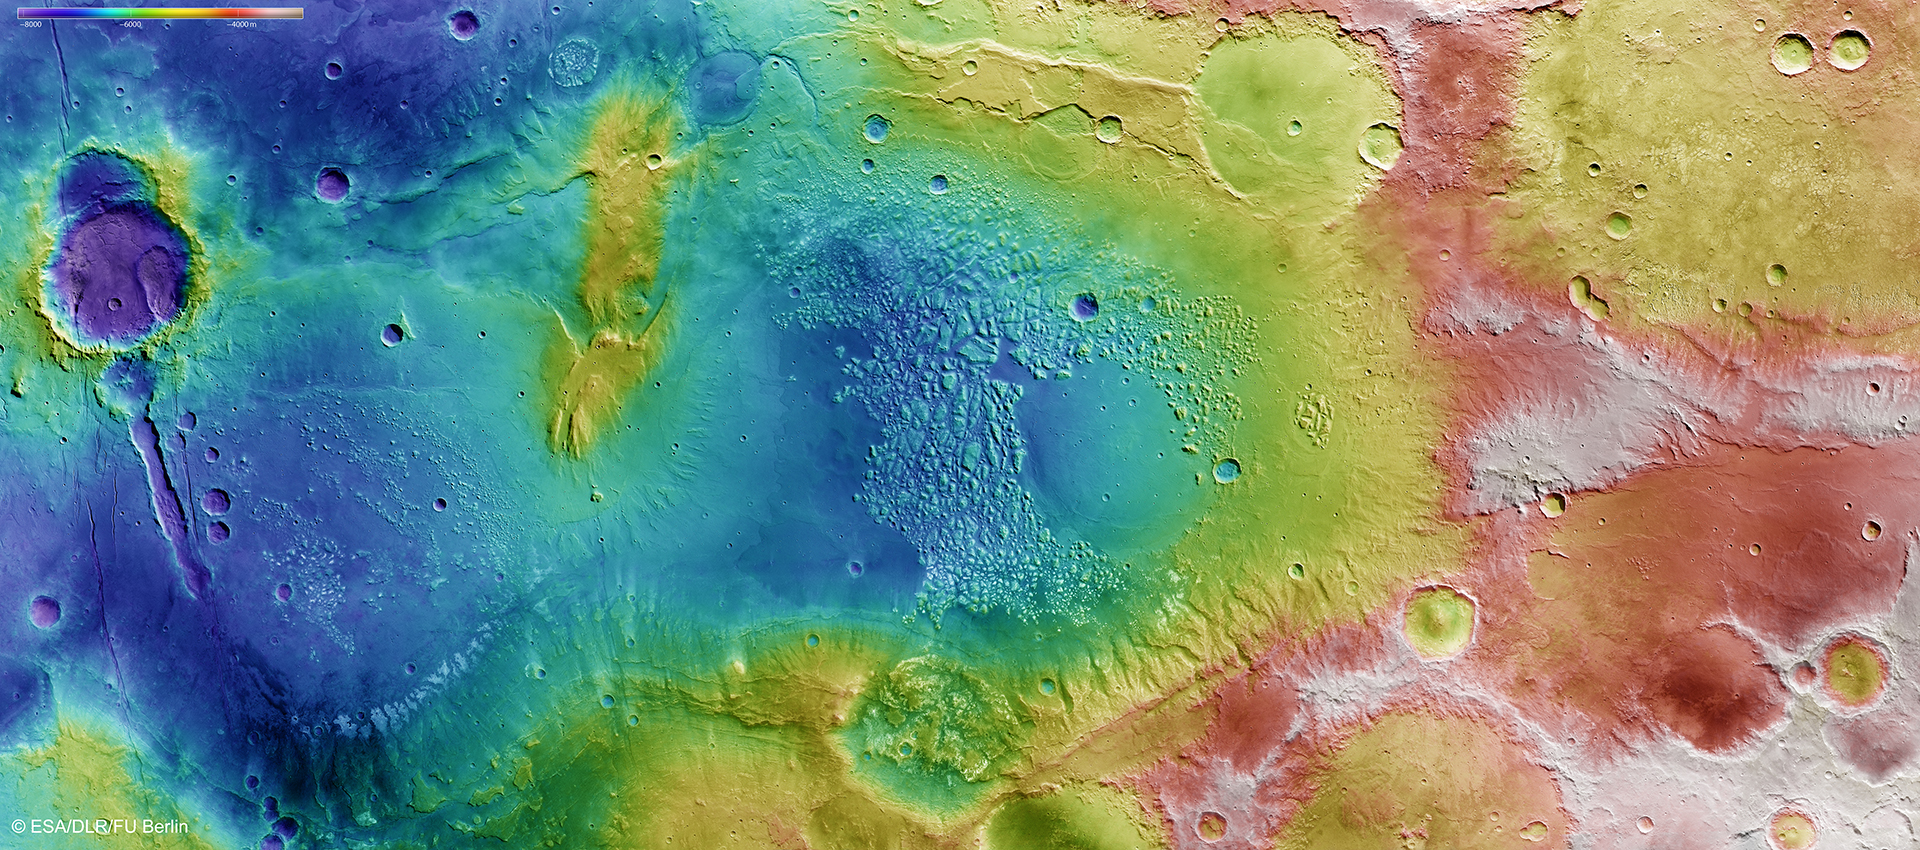
\includegraphics[width=\linewidth, trim={0 10cm 0 0}, clip]{Assets/Ancient_Atlantis.jpg}
\\Figura 1. Imágen con cotas del valle \textit{Ancient Atlantis}
\end{center}
El MEX es operado por la ESA desde su centro de operaciones en Darmstadt, Alemania. Desde ahí se analizan los datos recibidos así como también se monitorea cuidadosamente el estado del satélite, con el fin de planificar mejor las misiones de observación y evitar problemas en el suministro eléctrico.
\newline \par
Los operadores del MEX mantienen registros de su consumo de energía termal. La nave utiliza energía eléctrica, proveniente de paneles solares (o baterías, durante eclipses) no solo para alimentar los sensores y cámaras, sino también para mantener la temperatura del satélite dentro de rangos óptimos de funcionamiento. El resto de la energía que no se ocupa se puede derivar para realizar las transmisiones de datos.

\begin{center}
$E_{Telecomunicaciones} = E_{Generada} - E_{Sensores} - E_{Climatizacion}$
\end{center}

%\newline \par
El Mars Express Power Challenge se enfoca en predecir el consumo de energía destinada a la calefacción. El concurso provee datos de tres años (marcianos) como un set de entrenamiento y un cuarto año para pruebas. El éxito del concurso permitirá al MEX entregar información por periodos más largos de tiempo.

%High Resolution Stereo Camera (HRSC); 
%Energetic Neutral Atoms Analyser (ASPERA); 
%Planetary Fourier Spectrometer (PFS); 
%Visible and Infra Red Mineralogical Mapping Spectrometer (OMEGA); 
%Sub-Surface Sounding Radar Altimeter (MARSIS); 
%Mars Radio Science Experiment (MaRS); 
%Ultraviolet and Infrared Atmospheric Spectrometer (SPICAM);

%The Mars Express Orbiter will:
%image the entire surface at high resolution (10 metres/pixel) and selected areas at super resolution (2 metres/pixel);
%produce a map of the mineral composition of the surface at 100 metre resolution;
%map the composition of the atmosphere and determine its global circulation;
%determine the structure of the sub-surface to a depth of a few kilometres;
%determine the effect of the atmosphere on the surface;
%determine the interaction of the atmosphere with the solar wind.

%https://en.wikipedia.org/wiki/European_Space_Agency/

%http://www.esa.int/Our_Activities/Space_Science/Mars_Express/

%http://www.esa.int/spaceinimages/Images/2015/07/Ancient_Atlantis

%http://www.esa.int/spaceinvideos/Videos/2014/01/The_floodwaters_of_Mars

\end{document}